\documentclass[crop=false,10pt,ngerman]{standalone}
\usepackage{standard}
\begin{document}
  \section{Implementierung} % (fold)
  \label{sec:implementierung}

    \subsection{Repräsentation des Berechnungsgebietes} % (fold)
    \label{sub:repräsentation_des_berechnungsgebietes}
      Es handle sich bei $[\domain]\define\roundBrackets{\domain,\dirichletBoundary,\neumannBoundary,ν}$ wieder um ein Berechnungsgebiet.
      Die Implementierung einer Finite-Elemente-Methode verlangt die Diskretisierung von $[\domain]$, wie es in Abschnitt \ref{ssub:discretization-domain} beschrieben wurde.
      Das Ziel besteht darin, eine Klasse zu erstellen, die es ermöglicht, Berechnungsgebiete durch ein einfaches Dateiformat einzulesen, zu überprüfen und unter Umständen zu verfeinern.
      Eine weitere Klasse wird sich dann um die Konstruktion der Systemmatrizen und um die Berechnung des Zeitschrittes kümmern.
      Zunächst werden hierfür die grundlegendsten Strukturen eingeführt.
      Die simple Basisklasse \code{Domain\_base} im folgenden Quelltext definiert Kanten und Dreiecke, die auf Eckpunkte referenzieren.

      \inputCodeBlock[title=\code{Domain\_base}]{code/domain_base.cc}

      Die Basisstruktur \code{Domain\_base} wird im Namespace \code{Fem}, der auch für alle weiteren Codeausschnitte verwendet werden soll, konstruiert.
      In ihr werden die Strukturen \code{Edge} und \code{Primitive} für die Beschreibung der Kanten und Dreiecke deklariert.
      Die verschiedenen Konstruktoren und Zuweisungsoperatoren der Sprache C++ werden explizit durch den Compiler erzeugt.
      Der Destruktor wurde mit \code{virtual} gekennzeichnet, wie es für polymorphe Basisklassen angebracht ist \cite[S.~40~ff]{Meyers2008}.
      In den folgenden beiden Codeausschnitten werden die Strukturen \code{Edge} und \code{Primitive} implementiert.

      \inputCodeBlock[title=\code{Edge}]{code/edge.cc}
      \inputCodeBlock[title=\code{Primitive}]{code/primitive.cc}

      \code{Edge} und \code{Primitive} sind analog zueinander aufgebaut.
      Bei beiden handelt es sich um eine Spezialisierung von \code{std::array<int,...>} mit zwei oder drei Indizes.
      Diese Indizes werden später auf die Eckpunkte des Berechnungsgebietes verweisen.
      Die Konstruktoren stellen sicher, dass die Indizes sortiert übergeben werden.
      In beiden Fällen wird dabei eine explizite Formulierung des \enquote{Insertion Sort}-Verfahrens verwendet.
      Innerhalb der Datenstrukturen werden zwei weitere Datenstrukturen \code{Hash} und \code{Info} deklariert, die für die Verwendung mit der \enquote{Hash Map} \code{std::unordered\_map} vorgesehen sind.
      Eine \enquote{Hash Map} ist eine der effizientesten Varianten, um die Ränder eines Gebietes automatisch zu bestimmen.
      Zudem lässt sich durch diese sicher stellen, dass das konstruierte Gebiet fehlerfrei ist.

      Die eigentliche Datenstruktur \code{Domain} eines Berechnungsgebietes ist dann eine Spezialisierung der Basisklasse \code{Domain\_base} und nutzt demnach deren Kanten und Dreiecke.
      Der Datentyp der Eckpunkte wird durch ein \enquote{Template} variabel gehalten, sodass zum Beispiel der Austausch von Gleitkommazahlen mit einfacher Genauigkeit durch Gleitkommazahlen mit doppelter Genauigkeit kein Problem darstellt.
      Das Interface der Klasse ergibt sich aus Funktionen, um Daten zu lesen und fehlerfrei hinzuzufügen.
      Um dies auch in der Implementierung zu gewährleisten, speichert jede \enquote{Hash Map}, wie oft ein Dreieck oder eine Kante bereits hinzugefügt wurde.
      Auf der Basis dieser Zahl ist die Klasse dann in der Lage, zwischen Randkanten und inneren Kanten zu unterscheiden und fehlerhafte Berechnungsgebiete zu verhindern.
      Die folgenden beiden Codeausschnitte zeigen eine genaue Implementierung der wichtigsten Funktionen.
      In Abbildung \ref{fig:model-examples} sind als Beispiel verschiedene Testgebiete durch die Klasse \code{Domain} eingelesen und verarbeitet worden.

      \inputCodeBlock[title=\code{Domain}]{code/domain.cc}
      \inputCodeBlock[title=\code{Domain} Implementation]{code/domain_implementation.cc}

      \begin{figure}
        \begin{subfigure}[b]{0.24\textwidth}
          \center
          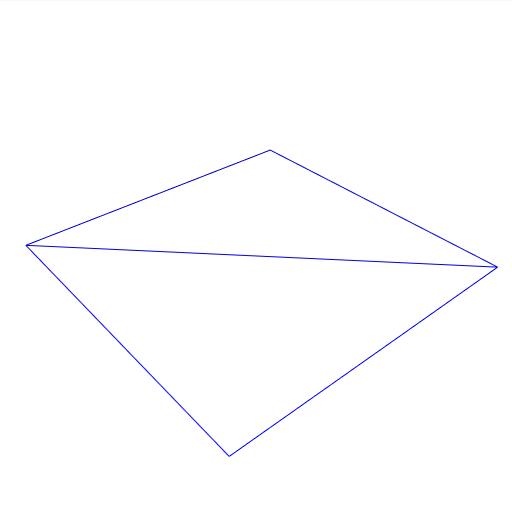
\includegraphics[trim={0 0 0 2cm},clip,width=0.95\textwidth]{images/model-quad-0.png}
          \caption{Quad}
        \end{subfigure}
        \begin{subfigure}[b]{0.24\textwidth}
          \center
          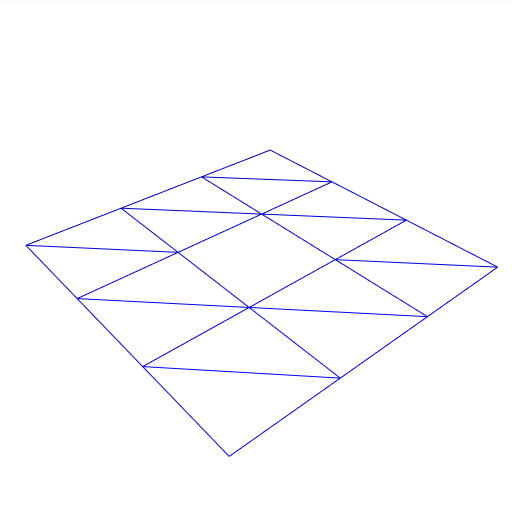
\includegraphics[trim={0 0 0 2cm},clip,width=0.95\textwidth]{images/model-ring-0.png}
          \caption{Ring}
        \end{subfigure}
        \begin{subfigure}[b]{0.24\textwidth}
          \center
          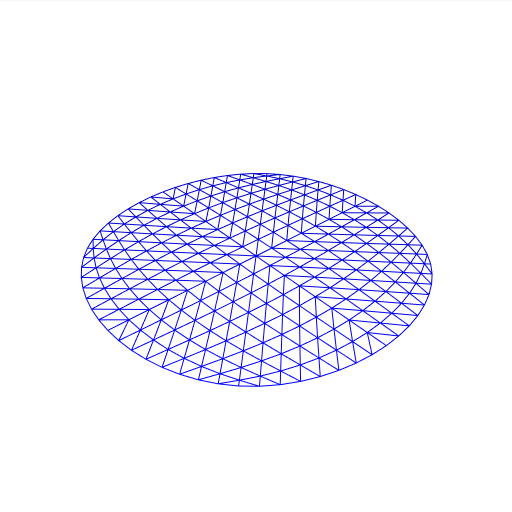
\includegraphics[trim={0 0 0 2cm},clip,width=0.95\textwidth]{images/model-circle-0.png}
          \caption{Curved}
        \end{subfigure}
        \begin{subfigure}[b]{0.24\textwidth}
          \center
          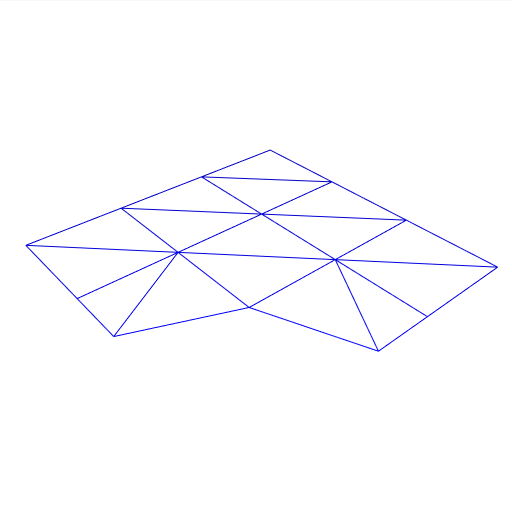
\includegraphics[trim={0 0 0 2cm},clip,width=0.95\textwidth]{images/model-test-0.png}
          \caption{Test}
        \end{subfigure}
        \caption[Beispiele verschiedener Berechnungsgebiete]{%
          Die Abbildungen zeigen verschiedene Beispiele für Berechnungsgebiete die mithilfe der Klasse \code{Domain} eingelesen und verarbeitet wurden.
        }
        \label{fig:model-examples}
      \end{figure}

      Für die späteren Messungen ist es von großem Nutzen, die Triangulierung eines Gebietes zu verfeinern.
      Hierfür enthält die Klasse \code{Domain} eine Funktion \code{subdivide}.
      Sie ermittelt für jede vorhandene Kante einen neuen Eckpunkt und fügt dann auf der Basis der alten Dreiecke neue feinere Dreiecke hinzu.
      Die unterteilten Kanten behalten dabei ihre Randeigenschaften.
      \inputCodeBlock[title=subdivide]{code/domain_implementation_subdivide.cc}

      Um ein Berechnungsgebiet außerhalb des Quelltextes leicht zu beschreiben, wurde ein Dateiformat definiert.
      Im folgenden ist ein Beispielmodell gezeigt.
      Hierbei steht \code{v} für die Definition eines Eckpunktes, \code{p} für die Definition eines Dreiecks, \code{q} für die Definition eines Vierecks, \code{d} für eine Dirichlet-Kante und \code{n} für eine Neumann-Kante.
      \begin{center}
        \noindent
        \begin{minipage}[b]{0.32\textwidth}
          \begin{tcolorbox}[titlerule=0.1pt,boxrule=0.5pt,arc=5pt,title={Zeile 1-13}]
            \lstinputlisting[style=standard,firstline=1,lastline=13]{code/model-test.txt}
          \end{tcolorbox}
        \end{minipage}
        \hfill
        \begin{minipage}[b]{0.32\textwidth}
          \begin{tcolorbox}[titlerule=0.1pt,boxrule=0.5pt,arc=5pt,title={Zeile 14-26}]
            \lstinputlisting[style=standard,firstline=14,lastline=26]{code/model-test.txt}
          \end{tcolorbox}
        \end{minipage}
        \hfill
        \begin{minipage}[b]{0.32\textwidth}
          \begin{tcolorbox}[titlerule=0.1pt,boxrule=0.5pt,arc=5pt,title={Zeile 27-39}]
            \lstinputlisting[style=standard,firstline=27,lastline=39]{code/model-test.txt}
          \end{tcolorbox}
        \end{minipage}
      \end{center}



      \begin{figure}[h]
        \begin{subfigure}[b]{0.24\textwidth}
          \center
          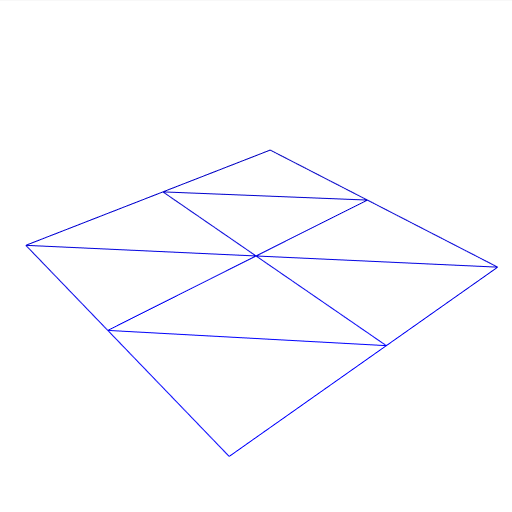
\includegraphics[trim={0 0 0 2cm},clip,width=0.95\textwidth]{images/model-quad-1.png}
          \caption{Quad}
        \end{subfigure}
        \begin{subfigure}[b]{0.24\textwidth}
          \center
          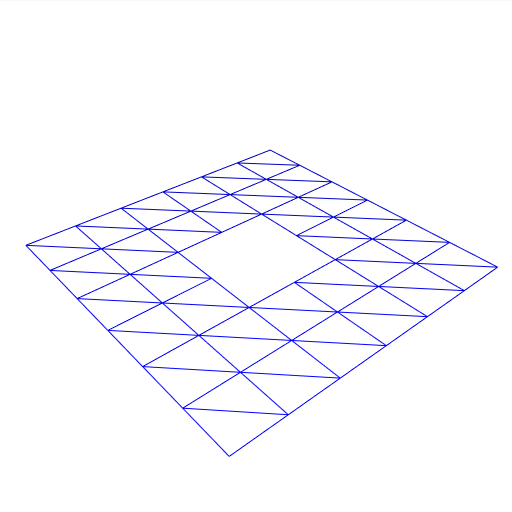
\includegraphics[trim={0 0 0 2cm},clip,width=0.95\textwidth]{images/model-ring-1.png}
          \caption{Ring}
        \end{subfigure}
        \begin{subfigure}[b]{0.24\textwidth}
          \center
          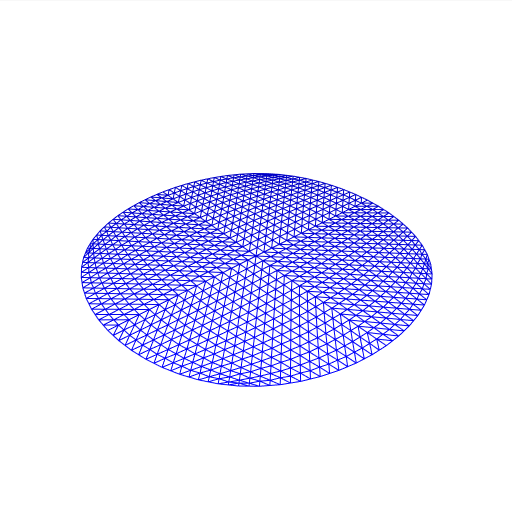
\includegraphics[trim={0 0 0 2cm},clip,width=0.95\textwidth]{images/model-circle-1.png}
          \caption{Curved}
        \end{subfigure}
        \begin{subfigure}[b]{0.24\textwidth}
          \center
          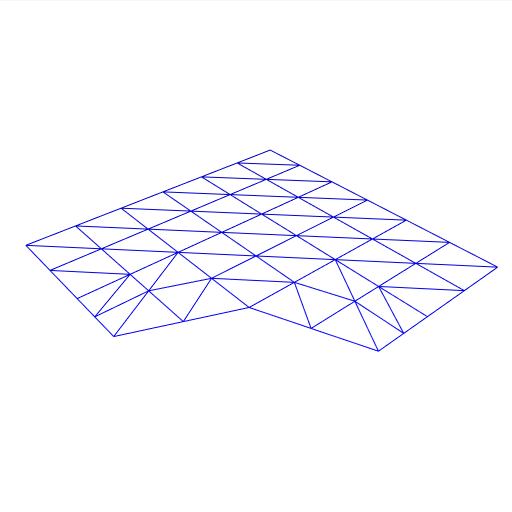
\includegraphics[trim={0 0 0 2cm},clip,width=0.95\textwidth]{images/model-test-1.png}
          \caption{Test}
        \end{subfigure}
      \end{figure}
    % subsection repräsentation_des_berechnungsgebietes (end)

    \subsection{Aufbau des Systems} % (fold)
    \label{sub:aufbau_des_systems}
      Ein System zur Lösung der Wellengleichung soll zunächst auf der CPU implementiert werden.
      Hierfür wird die Klasse \code{Cpu\_wave\_system} eingeführt.
      Sie verwendet die Bibliothek \enquote{Eigen} für alle grundlegenden Matrix-Vektor-Operationen \cite{Eigen2018}.
      \inputCodeBlock[title=Wave system]{code/cpu_wave_system.cc}
      Das Interface des Systems besteht grundlegend aus einer Funktion \code{initial\_state}, die es ermöglicht, die Anfangsbedingungen zu setzen, und einer Funktion \code{advance}, die das gesamte System einen Zeitschritt voranbringt.
      Systemmatrizen der Finite-Elemente-Methode, sowie die Welle und deren Ableitungen, werden zwischengespeichert, um unnötige Berechnungsschritte zu verhindern.
      Des Weiteren sollen bei der Konstruktion des Systems Eckpunkte, die auf dem Rand des Gebietes liegen, von den inneren Eckpunkten separiert werden.
      Hierfür wird das Array der Eckpunkte innerhalb des Systems permutiert.
      Die Permutation wird für den Zugriff von außen gespeichert.
      Im weiteren Verlauf sollen die Neumann-Randbedingungen auf Null gesetzt werden, sodass die Konstruktion der Neumann-Rand-Matrix nicht notwendig ist.
      Die Neumann-Rand-Matrix ließe sich aber analog zu den anderen Systemmatrizen durch eine Iteration über alle Neumann-Kanten konstruieren.

      Auf der GPU ist die Verwendung von \enquote{Eigen} nicht möglich.
      Aus diesem Grund ist eine explizite Implementierung des CSR-Formates auf dem DRAM der GPU nötig.
      Um den Zugriff auf die Daten in CUDA zu ermöglichen, werden Zeiger definiert.
      Das Interface der Klasse \code{Gpu\_wave\_system} unterscheidet sich im Wesentlichen nicht von dem der Klasse \code{Cpu\_wave\_system}.
      Möchte man jedoch die Welle auslesen, so müssen deren Daten vom DRAM wieder in den RAM übertragen werden.
      Eben deshalb wird eine Funktion \code{copy\_wave} deklariert.

      \inputCodeBlock[title = GPU Wave system]{code/gpu_wave_system.cc}
    % subsection aufbau_des_systems (end)

    \subsection{Konstruktion der Systemmatrizen} % (fold)
    \label{sub:konstruktion_der_mass_und_stiffness_matrix}
      Die Konstruktion der Systemmatrizen muss in dieser Arbeit für jedes Berechnungsgebiet nur ein einziges Mal ausgeführt werden.
      Aus diesem Grund soll hier auf die Implementierung einer parallelisierten Methode auf der GPU verzichtet werden.

      Für eine effiziente Berechnung des Zeitschrittes sollen vor der eigentlichen Konstruktion alle Eckpunkte durch \enquote{Counting Sort} sortiert werden.
      Das folgende Schema veranschaulicht diese Überlegung und zeigt zudem die Bereiche der Indizes an, auf die die unterschiedlichen Systemmatrizen zugreifen.
      Die Sortierung der Eckpunkte steigert die Performance des Matrix-Vektor-Produktes, welches nun bei der Berechnung linear auf dem Speicher arbeitet, und vereinfacht das Interface.
      \begin{align*}
        &\,\framebox[0.81\textwidth]{\footnotesize ungeordnete Eckpunkte} \\
        &\makebox[0.81\textwidth]{\hfill $\downarrow \text{\footnotesize Counting Sort} \downarrow$ \hfill}\\
        & \underbrace{\framebox[0.3\textwidth]{\footnotesize innere Eckpunkte}\underbrace{\framebox[0.25\textwidth]{\footnotesize Neumann-Eckpunkte}}_{\text{Neumann-Rand-Matrix}}}_{\text{innere Matrix}} \underbrace{\framebox[0.25\textwidth]{\footnotesize Dirichlet-Eckpunkte}}_{\text{Dirichlet-Rand-Matrix}}
      \end{align*}
      Für die Simulation der Wellengleichung mit natürlichem Neumann-Rand werden vier Systemmatrizen benötigt.
      Diese teilen sich auf in die inneren Matrizen, die die Wechselwirkung freier Eckpunkte untereinander beschreiben, und Randmatrizen, die die Wechselwirkung des Dirichlet-Randes mit inneren Eckpunkten beschreiben.
      % Zunächst werden die Eckpunkte auf einem Dirichlet-Rand markiert.
      % Auf der Basis dieser Markierung lässt sich die Permutation konstruieren.
      Nach der Berechnung der Permutation durch \enquote{Counting Sort}, wird über alle Dreiecke iteriert.
      Jedes Dreieck liefert die Matrix eines finiten Elementes.
      Diese Matrizen werden entsprechend dem Standardverfahren von \enquote{Eigen} akkumuliert und zu den Systemmatrizen zusammengesetzt \cite{Eigen2018}.
      \inputCodeBlock[title = System construction]{code/cpu_wave_system_constructor.cc}

      Für die GPU müssen die auf der CPU konstruierten Daten der dünnbesetzten Matrizen noch auf den DRAM übertragen werden.
      Nützlich dabei ist, dass die beiden inneren Matrizen das gleiche Muster aufweisen.
      Ebenso gilt dies für die beiden Randmatrizen.
      Die vier CSR-Matrizen lassen sich also zu zwei kompletten CSR-Matrizen und zwei zusätzlichen Wertearrays komprimieren.
      Während der Konstruktion wird zudem die maximale Anzahl von Threads auf einem Block der verwendeten GPU ausgelesen.
      Mithilfe dieses Wertes wird eine optimale Anzahl von Threads auf den verschiedenen Blocks der GPU generiert.
      \inputCodeBlock[title = System construction]{code/gpu_wave_system_constructor.cc}

      Da die Daten auf dem DRAM über herkömmliche Zeiger verwaltet werden, muss der Destruktor der Klasse den allozierten Speicher auf dem DRAM wieder freigeben.
      \inputCodeBlock[title = System construction]{code/gpu_wave_system_destructor.cc}

      Die Funktionen, um die Anfangsdaten zu setzen und die Wellendaten auszulesen, müssen ebenfalls die Daten zwischen dem RAM und dem DRAM transportieren.
      Dies funktioniert analog wieder mit \code{cudaMemcpy} oder \code{thrust::copy}.
      % \inputCodeBlock[title = System construction]{code/gpu_wave_system_accessors.cc}
    % subsection konstruktion_der_mass_und_stiffness_matrix (end)

    \subsection{Berechnung eines Zeitschrittes} % (fold)
    \label{sub:time-step-computation}
      Die Berechnung eines weiteren Zeitschrittes erfordert die Konstruktion der rechten Seite des linearen Gleichungssystems.
      Mithilfe des in \enquote{Eigen} implementierten CG-Verfahrens wird dann die Ableitung der Welle zum neuen Zeitpunkt berechnet.
      Anschließend kann mit dieser Ableitung die neue Welle generiert werden.
      \inputCodeBlock[title = CPU Wave System advance]{code/cpu_wave_system_advance.cc}

      Um den Lösungsalgorithmus auf der GPU zu programmieren, soll zunächst das CG-Verfahren auf der CPU implementiert werden.
      Der folgende Quelltext zeigt dies.
      \inputCodeBlock[title = Conjugate Gradient]{code/cpu_conjugate_gradient.cc}
      Innerhalb der GPU wird nun genau wie auf der CPU zuerst die rechte Seite des linearen Gleichungssystems konstruiert und dann ein CG-Verfahren angewendet.
      Um die Implementierung einfacher zu gestalten, wurde \enquote{Thrust} verwendet \cite{cuda2018}.
      \inputCodeBlock[title = GPU Wave System advance]{code/gpu_wave_system_advance.cc}
      Innerhalb des Codes wird ein Kernel definiert, der die Matrix-Vektor-Multiplikation des CSR-Formates auf der GPU parallelisiert.
      Des Weiteren wurden zwei Funktoren \code{axpy\_functor} und \code{axpby\_functor} verwendet, die die typischen BLAS Routinen darstellen.
      \inputCodeBlock[title = GPU Kernel]{code/gpu_wave_system_kernel.cc}
    % subsection konstruktion_des_linearen_gleichungssystems (end)

    \subsection{Visualisierung} % (fold)
    \label{sub:visualisierung}

      \begin{figure}[p]
        \center
        \begin{subfigure}[b]{0.24\textwidth}
          \center
          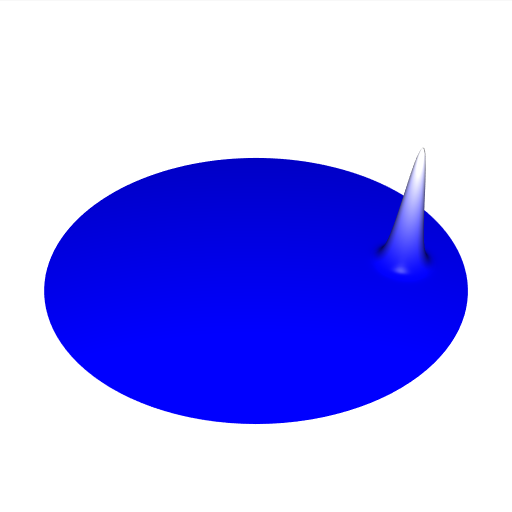
\includegraphics[trim={1.5cm 3.05cm 1.5cm 5.2cm},clip,width=0.95\textwidth]{images/circle_wave_0.png}
          \caption{}
        \end{subfigure}
        \begin{subfigure}[b]{0.24\textwidth}
          \center
          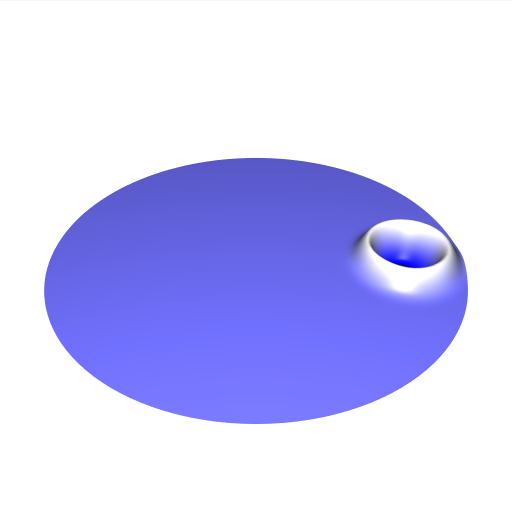
\includegraphics[trim={1.5cm 3.05cm 1.5cm 5.2cm},clip,width=0.95\textwidth]{images/circle_wave_1.png}
          \caption{}
        \end{subfigure}
        \begin{subfigure}[b]{0.24\textwidth}
          \center
          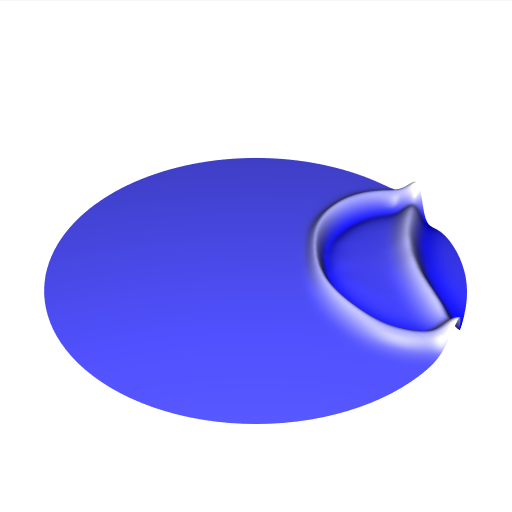
\includegraphics[trim={1.5cm 3.05cm 1.5cm 5.2cm},clip,width=0.95\textwidth]{images/circle_wave_2.png}
          \caption{}
        \end{subfigure}
        \begin{subfigure}[b]{0.24\textwidth}
          \center
          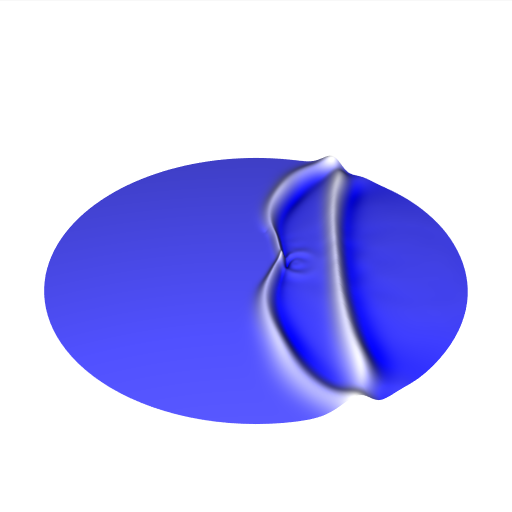
\includegraphics[trim={1.5cm 3.05cm 1.5cm 5.2cm},clip,width=0.95\textwidth]{images/circle_wave_3.png}
          \caption{}
        \end{subfigure}

        \begin{subfigure}[b]{0.24\textwidth}
          \center
          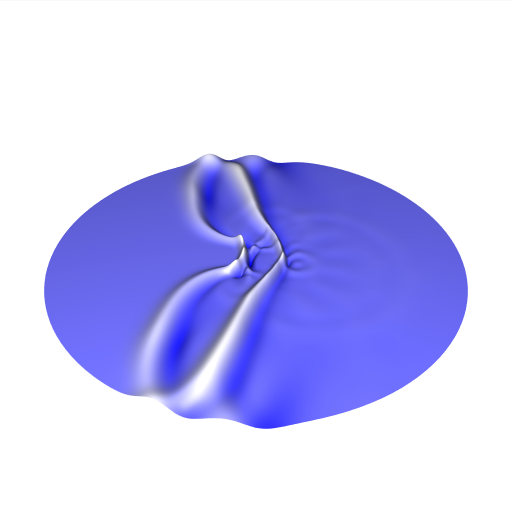
\includegraphics[trim={1.5cm 3.05cm 1.5cm 5.2cm},clip,width=0.95\textwidth]{images/circle_wave_4.png}
          \caption{}
        \end{subfigure}
        \begin{subfigure}[b]{0.24\textwidth}
          \center
          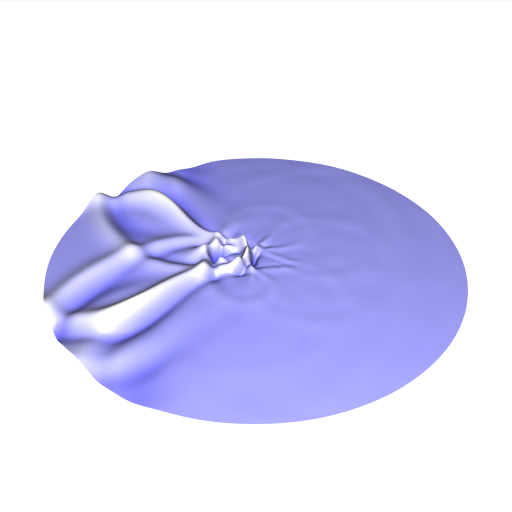
\includegraphics[trim={1.5cm 3.05cm 1.5cm 5.2cm},clip,width=0.95\textwidth]{images/circle_wave_5.png}
          \caption{}
        \end{subfigure}
        \begin{subfigure}[b]{0.24\textwidth}
          \center
          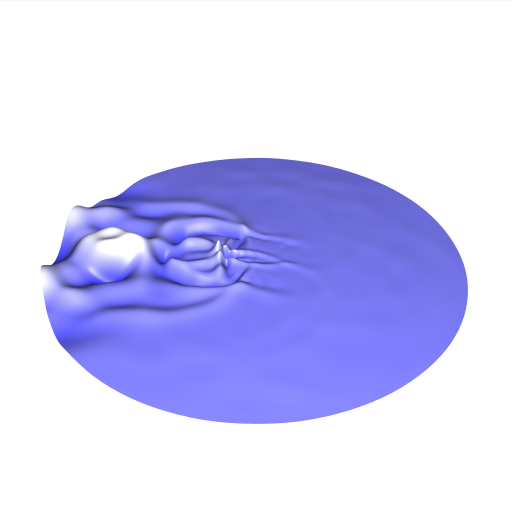
\includegraphics[trim={1.5cm 3.05cm 1.5cm 5.2cm},clip,width=0.95\textwidth]{images/circle_wave_6.png}
          \caption{}
        \end{subfigure}
        \begin{subfigure}[b]{0.24\textwidth}
          \center
          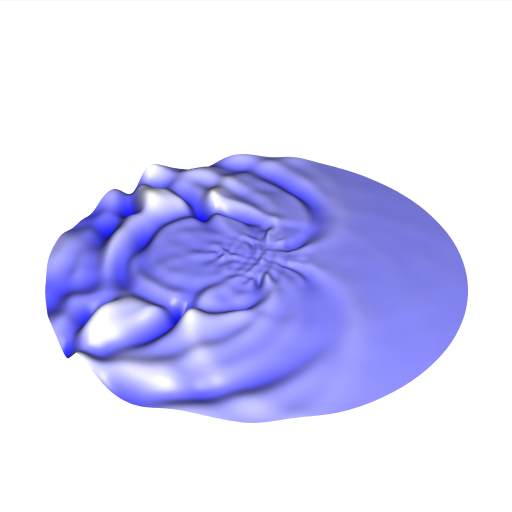
\includegraphics[trim={1.5cm 3.05cm 1.5cm 5.2cm},clip,width=0.95\textwidth]{images/circle_wave_7.png}
          \caption{}
        \end{subfigure}
        \caption[Wellensimulation auf einem Kreis]{%
          Die Abbildungen zeigen die Zeitevolution einer Simulation der Wellengleichung auf dem Gebiet \enquote{Circle}.
          Bei diesem Berechnungsgebiet handelt es sich um einen Kreis mit Neumann-Randbedingungen.
          Die spezielle Art der Triangulierung verursacht hier in der Nähe des Mittelpunktes numerische Fehler.
          Bereits im vierten Bild entsteht im Zentrum der Welle ein Knick, der das Ergebnis verfälscht.
        }
        \label{fig:circle-wave}
      \end{figure}

      Für die Simulation der Wellengleichung reicht es an sich aus, das CG-Verfahren zu verwenden und das lineare Gleichungssystem zu lösen.
      Bei der berechneten Lösung handelt es sich um einen Vektor, der die Werte der Wellenfunktion über den einzelnen Eckpunkten speichert.
      Durch automatisierte Testverfahren ist der Computer teilweise in der Lage, die Ergebnisse auf Fehler zu überprüfen.
      Allerdings verändert sich eine Welle auf einem berandeten Gebiet mit fortschreitender Zeit auf immer komplexere Art und Weise.
      Aus diesem Grund stellt das subjektive Empfinden des Programmierers beziehungsweise Modellierers, welches bei der Betrachtung der Welle entsteht, ein weiteres Testverfahren dar, um die Korrektheit des Algorithmus unter gewissen Einschränkungen zu gewährleisten.
      Die Eigenschaften einer visualisierten Wellenfunktion sind für einen Menschen leichter nachzuvollziehen als eine reine Ansammlung von Daten.
      Abbildung \ref{fig:circle-wave} zeigt zum Beispiel numerische Fehler einer Wellensimulation, die durch die spezielle Form des Gitters auftreten und schwer durch automatisierte Tests zu finden sind.

      \begin{figure}[p]
        \center
        \begin{subfigure}[b]{0.24\textwidth}
          \center
          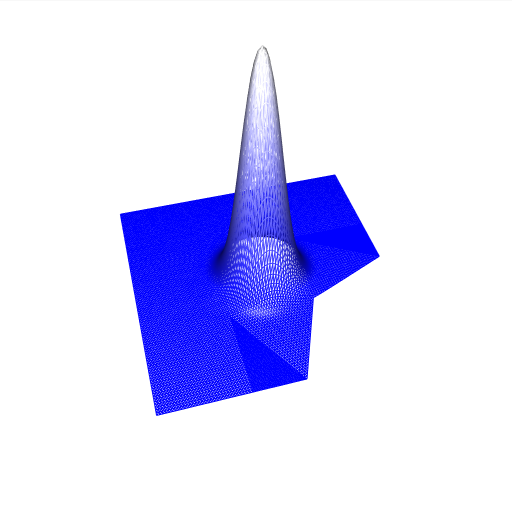
\includegraphics[trim={4cm 1.2cm 4.5cm 1.5cm},clip,width=0.95\textwidth]{images/test_wave_0.png}
          \caption{}
        \end{subfigure}
        \begin{subfigure}[b]{0.24\textwidth}
          \center
          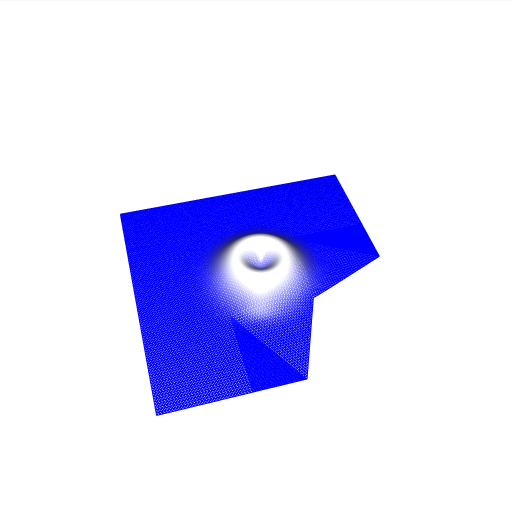
\includegraphics[trim={4cm 1.2cm 4.5cm 1.5cm},clip,width=0.95\textwidth]{images/test_wave_1.png}
          \caption{}
        \end{subfigure}
        \begin{subfigure}[b]{0.24\textwidth}
          \center
          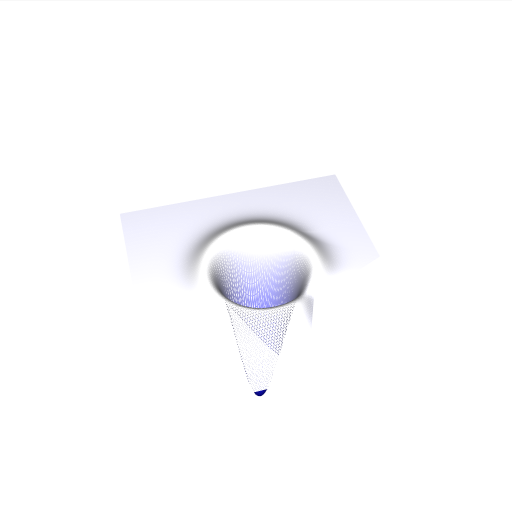
\includegraphics[trim={4cm 1.2cm 4.5cm 1.5cm},clip,width=0.95\textwidth]{images/test_wave_2.png}
          \caption{}
        \end{subfigure}
        \begin{subfigure}[b]{0.24\textwidth}
          \center
          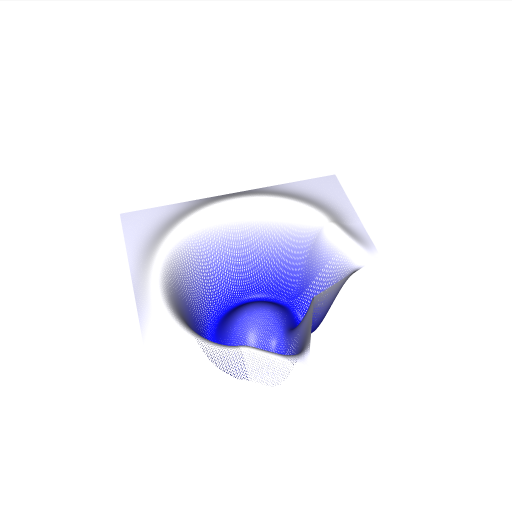
\includegraphics[trim={4cm 1.2cm 4.5cm 1.5cm},clip,width=0.95\textwidth]{images/test_wave_3.png}
          \caption{}
        \end{subfigure}

        \begin{subfigure}[b]{0.24\textwidth}
          \center
          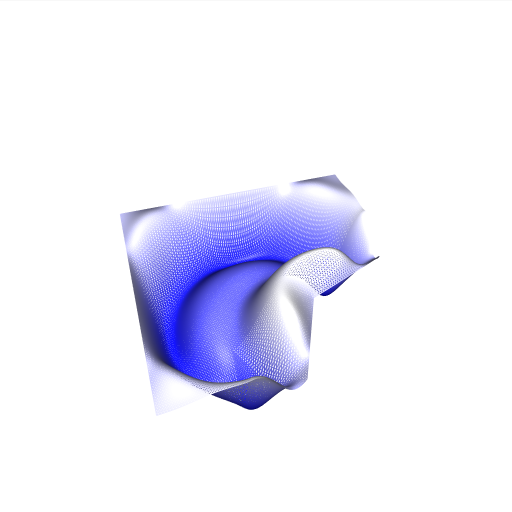
\includegraphics[trim={4cm 1.2cm 4.5cm 1.5cm},clip,width=0.95\textwidth]{images/test_wave_4.png}
          \caption{}
        \end{subfigure}
        \begin{subfigure}[b]{0.24\textwidth}
          \center
          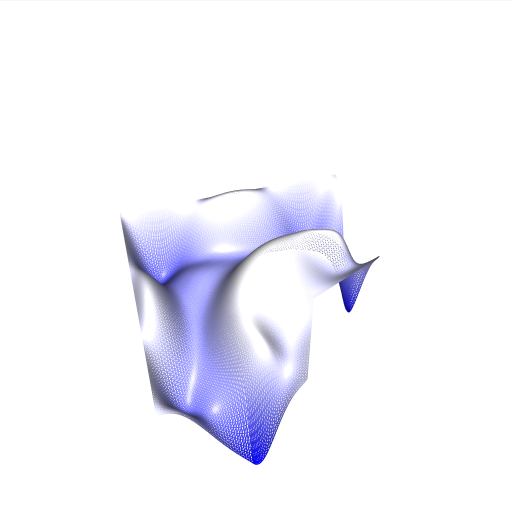
\includegraphics[trim={4cm 1.2cm 4.5cm 1.5cm},clip,width=0.95\textwidth]{images/test_wave_5.png}
          \caption{}
        \end{subfigure}
        \begin{subfigure}[b]{0.24\textwidth}
          \center
          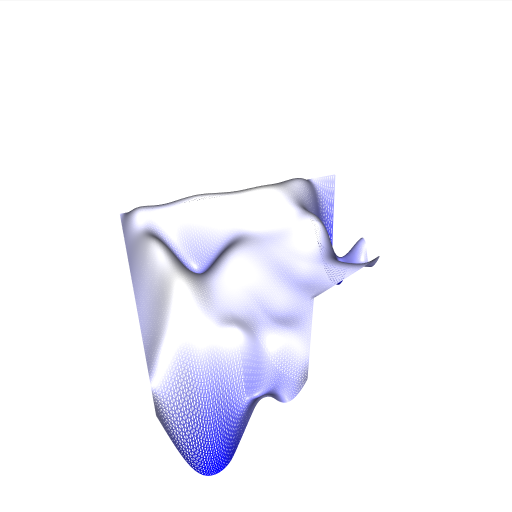
\includegraphics[trim={4cm 1.2cm 4.5cm 1.5cm},clip,width=0.95\textwidth]{images/test_wave_6.png}
          \caption{}
        \end{subfigure}
        \begin{subfigure}[b]{0.24\textwidth}
          \center
          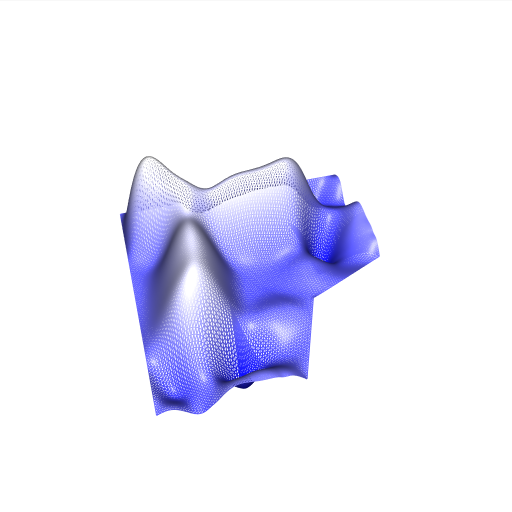
\includegraphics[trim={4cm 1.2cm 4.5cm 1.5cm},clip,width=0.95\textwidth]{images/test_wave_7.png}
          \caption{}
        \end{subfigure}
        \caption[Wellensimulation auf dem Testgebiet]{%
          Die Abbildungen zeigen die Zeitevolution einer Simulation der Wellengleichung auf dem Gebiet \enquote{Test}.
          Dieses Gebiet wurde in \cite{Alberty1998} beschrieben.
          Es wurden dabei gemischte Randbedingungen gewählt.
        }
        \label{fig:test-wave}
      \end{figure}

      \begin{figure}[p]
        \center
        \begin{subfigure}[b]{0.24\textwidth}
          \center
          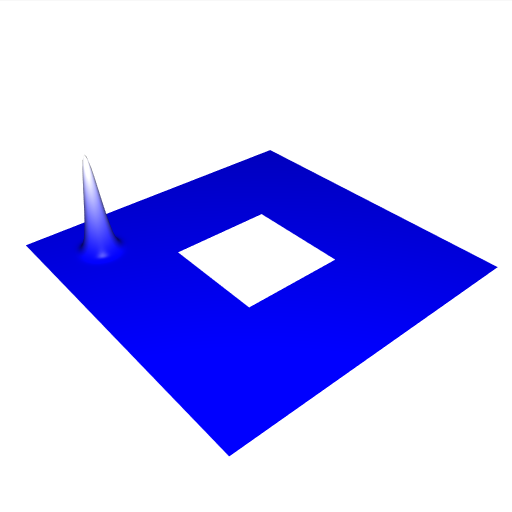
\includegraphics[trim={0.9cm 1.8cm 0.5cm 5cm},clip,width=0.95\textwidth]{images/ring_wave_0.png}
          \caption{}
        \end{subfigure}
        \begin{subfigure}[b]{0.24\textwidth}
          \center
          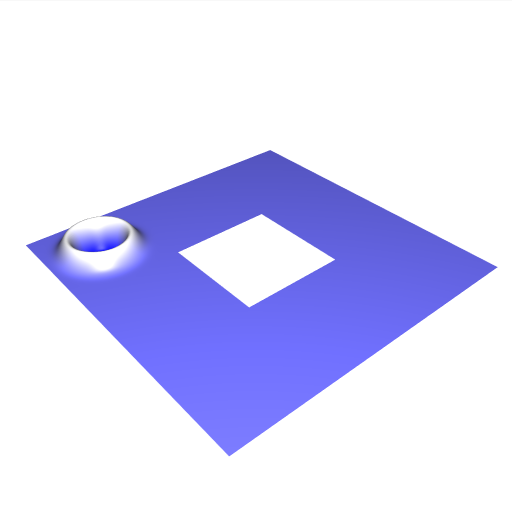
\includegraphics[trim={0.9cm 1.8cm 0.5cm 5cm},clip,width=0.95\textwidth]{images/ring_wave_1.png}
          \caption{}
        \end{subfigure}
        \begin{subfigure}[b]{0.24\textwidth}
          \center
          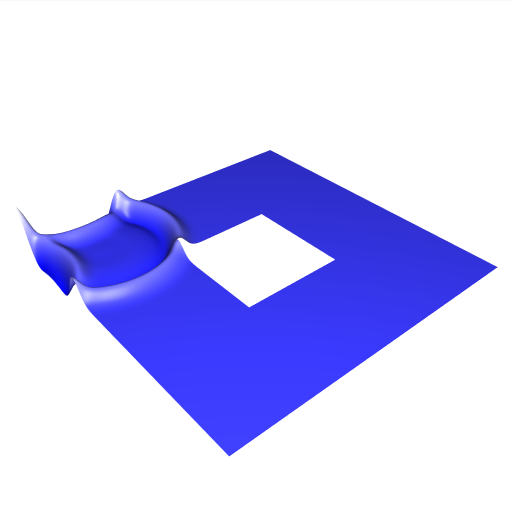
\includegraphics[trim={0.9cm 1.8cm 0.5cm 5cm},clip,width=0.95\textwidth]{images/ring_wave_2.png}
          \caption{}
        \end{subfigure}
        \begin{subfigure}[b]{0.24\textwidth}
          \center
          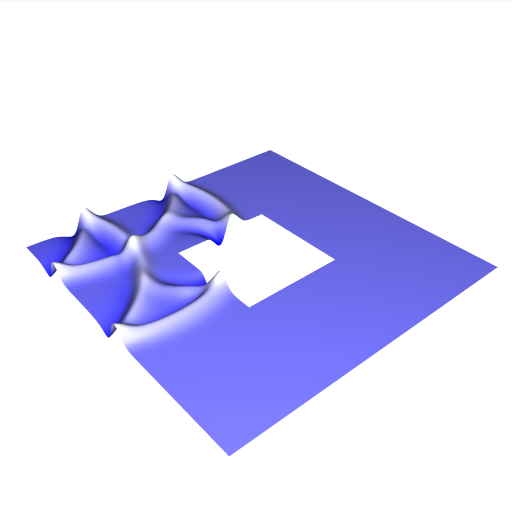
\includegraphics[trim={0.9cm 1.8cm 0.5cm 5cm},clip,width=0.95\textwidth]{images/ring_wave_3.png}
          \caption{}
        \end{subfigure}

        \begin{subfigure}[b]{0.24\textwidth}
          \center
          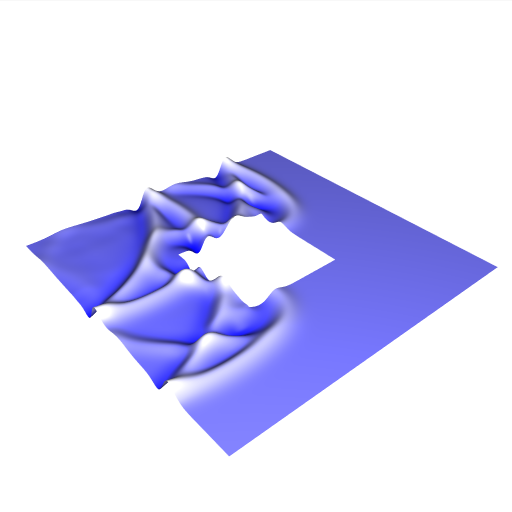
\includegraphics[trim={0.9cm 1.8cm 0.5cm 5cm},clip,width=0.95\textwidth]{images/ring_wave_4.png}
          \caption{}
        \end{subfigure}
        \begin{subfigure}[b]{0.24\textwidth}
          \center
          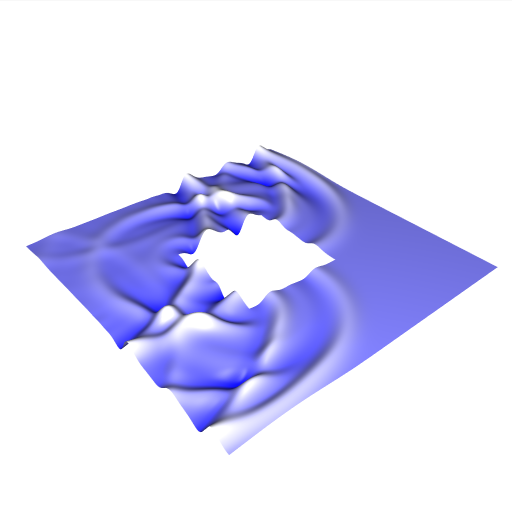
\includegraphics[trim={0.9cm 1.8cm 0.5cm 5cm},clip,width=0.95\textwidth]{images/ring_wave_5.png}
          \caption{}
        \end{subfigure}
        \begin{subfigure}[b]{0.24\textwidth}
          \center
          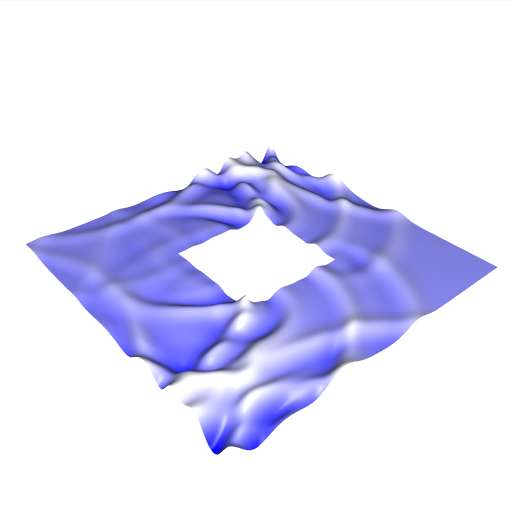
\includegraphics[trim={0.9cm 1.8cm 0.5cm 5cm},clip,width=0.95\textwidth]{images/ring_wave_6.png}
          \caption{}
        \end{subfigure}
        \begin{subfigure}[b]{0.24\textwidth}
          \center
          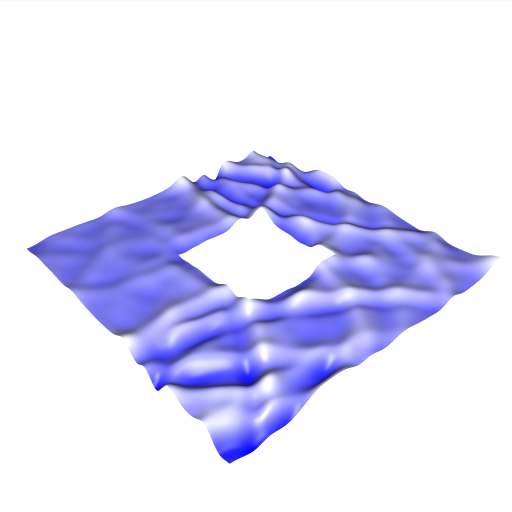
\includegraphics[trim={0.9cm 1.8cm 0.5cm 5cm},clip,width=0.95\textwidth]{images/ring_wave_7.png}
          \caption{}
        \end{subfigure}
        \caption[Wellensimulation auf einem quadratischen Ring]{%
          Die Abbildungen zeigen die Zeitevolution einer Simulation der Wellengleichung auf dem Gebiet \enquote{Ring}.
          Es handelt sich dabei um einen quadratischen Ring mit Neumann-Randbedingungen.
          Es lassen sich hier typische Effekte, wie Beugung und Interferenz, beobachten.
        }
        \label{fig:ring-wave}
      \end{figure}

      \begin{figure}[p]
        \center
        \begin{subfigure}[b]{0.24\textwidth}
          \center
          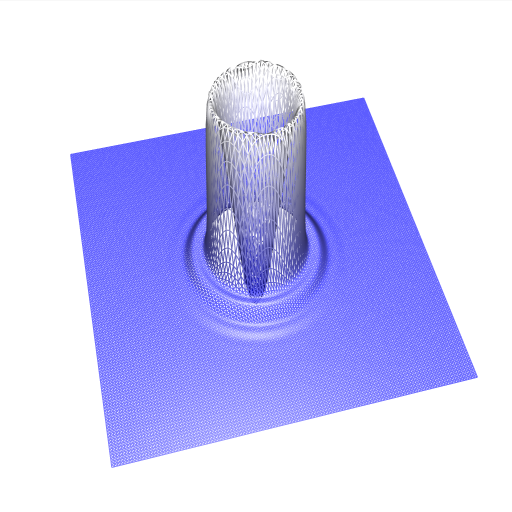
\includegraphics[trim={2cm 1.5cm 1.2cm 1.0cm},clip,width=0.95\textwidth]{images/quad_wave_0.png}
          \caption{}
        \end{subfigure}
        \begin{subfigure}[b]{0.24\textwidth}
          \center
          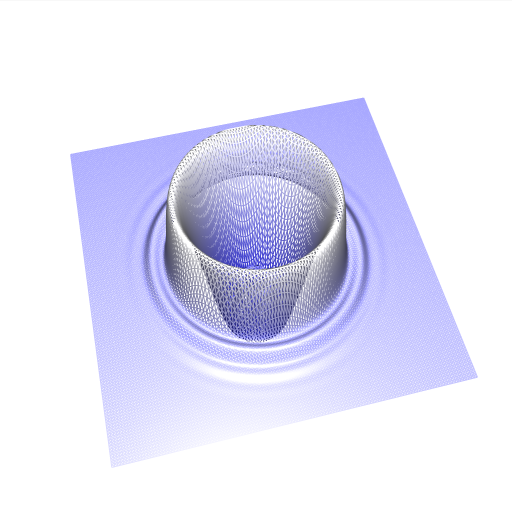
\includegraphics[trim={2cm 1.5cm 1.2cm 1.0cm},clip,width=0.95\textwidth]{images/quad_wave_1.png}
          \caption{}
        \end{subfigure}
        \begin{subfigure}[b]{0.24\textwidth}
          \center
          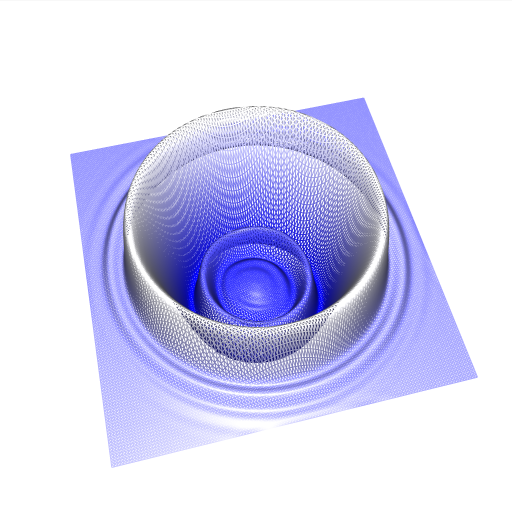
\includegraphics[trim={2cm 1.5cm 1.2cm 1.0cm},clip,width=0.95\textwidth]{images/quad_wave_2.png}
          \caption{}
        \end{subfigure}
        \begin{subfigure}[b]{0.24\textwidth}
          \center
          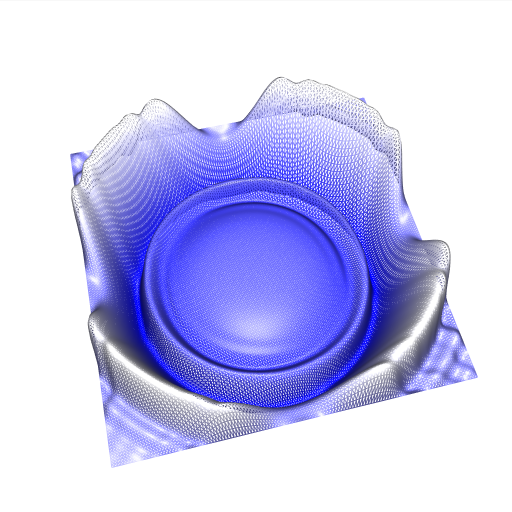
\includegraphics[trim={2cm 1.5cm 1.2cm 1.0cm},clip,width=0.95\textwidth]{images/quad_wave_3.png}
          \caption{}
        \end{subfigure}

        \begin{subfigure}[b]{0.24\textwidth}
          \center
          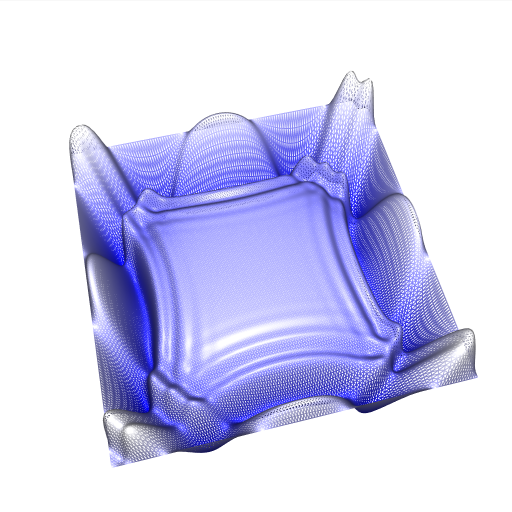
\includegraphics[trim={2cm 1.5cm 1.2cm 1.0cm},clip,width=0.95\textwidth]{images/quad_wave_4.png}
          \caption{}
        \end{subfigure}
        \begin{subfigure}[b]{0.24\textwidth}
          \center
          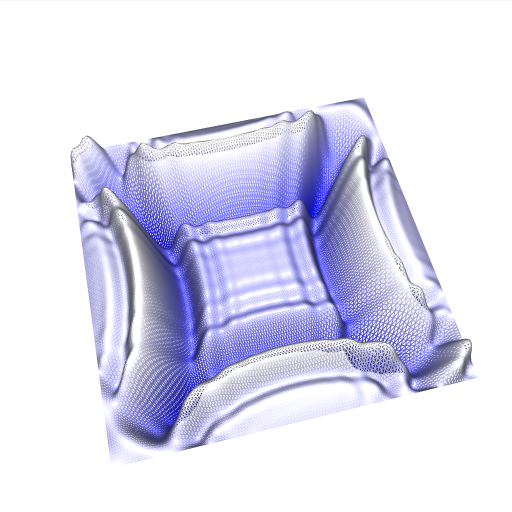
\includegraphics[trim={2cm 1.5cm 1.2cm 1.0cm},clip,width=0.95\textwidth]{images/quad_wave_5.png}
          \caption{}
        \end{subfigure}
        \begin{subfigure}[b]{0.24\textwidth}
          \center
          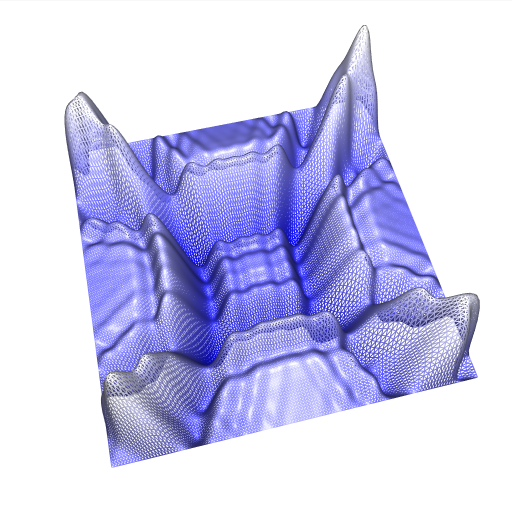
\includegraphics[trim={2cm 1.5cm 1.2cm 1.0cm},clip,width=0.95\textwidth]{images/quad_wave_6.png}
          \caption{}
        \end{subfigure}
        \begin{subfigure}[b]{0.24\textwidth}
          \center
          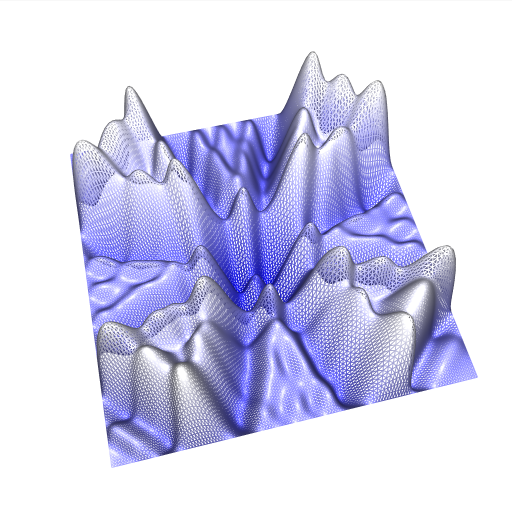
\includegraphics[trim={2cm 1.5cm 1.2cm 1.0cm},clip,width=0.95\textwidth]{images/quad_wave_7.png}
          \caption{}
        \end{subfigure}
        \caption[Wellensimulation auf einem quadratischen Gebiet]{%
          Die Abbildungen zeigen die Zeitevolution einer Simulation der Wellengleichung auf dem Gebiet \enquote{Quad}.
          Es handelt sich um ein quadratisches Berechnungsgebiet mit Dirichlet-Randbedingungen.
        }
        \label{fig:quad-wave}
      \end{figure}

      Die Verwendung von OpenGL ermöglicht die dreidimensionale Darstellung von Objekten, die durch Dreiecke im dreidimensionalen Raum diskretisiert wurden.
      Die finiten Elemente des Berechnungsgebietes sind grundsätzlich im zweidimensionalen Raum definiert.
      Deshalb soll eine dritte Koordinate den Wert der Wellenfunktion an der entsprechenden Stelle eines jeden Eckpunktes beschreiben.
      Dies führt dazu, dass sich das angezeigte Berechnungsgebiet entsprechend der Welle verformt, sodass dessen Aussehen mit der einer Wasseroberfläche verglichen werden kann.
      Um den Eindruck zu verstärken, wird für jeden Eckpunkt auf der Basis der benachbarten Dreiecke eine Normale berechnet, die das Gebiet wie eine differenzierbare Fläche erscheinen lässt.
      Weiterhin wird den einzelnen Werten der Welle noch eine Farbe zugewiesen.
      Damit fällt es dem Benutzer einfacher auch kleine Unterschiede wahrzunehmen.
      Die Abbildungen \ref{fig:test-wave}, \ref{fig:quad-wave}, \ref{fig:ring-wave} und \ref{fig:circle-wave} zeigen die Visualisierung der berechneten Welle über dem entsprechenden Gebiet anhand ausgewählter Beispiele.

    % subsection visualisierung (end)
  % section implementierung (end)
\end{document}